% Options for packages loaded elsewhere
\PassOptionsToPackage{unicode}{hyperref}
\PassOptionsToPackage{hyphens}{url}
%
\documentclass[10pt,a4paper]{article}
\usepackage[left=25mm,right=25mm]{geometry}
\usepackage{amsmath}
\usepackage{amsfonts}
\usepackage{amssymb}

\usepackage{amsmath,amssymb}
\usepackage{lmodern}
\usepackage{iftex}
\ifPDFTeX
  \usepackage[T1]{fontenc}
  \usepackage[utf8]{inputenc}
  \usepackage{textcomp} % provide euro and other symbols
\else % if luatex or xetex
  \usepackage{unicode-math}
  \defaultfontfeatures{Scale=MatchLowercase}
  \defaultfontfeatures[\rmfamily]{Ligatures=TeX,Scale=1}
\fi
% Use upquote if available, for straight quotes in verbatim environments
\IfFileExists{upquote.sty}{\usepackage{upquote}}{}
\IfFileExists{microtype.sty}{% use microtype if available
  \usepackage[]{microtype}
  \UseMicrotypeSet[protrusion]{basicmath} % disable protrusion for tt fonts
}{}
\makeatletter
\@ifundefined{KOMAClassName}{% if non-KOMA class
  \IfFileExists{parskip.sty}{%
    \usepackage{parskip}
  }{% else
    \setlength{\parindent}{0pt}
    \setlength{\parskip}{6pt plus 2pt minus 1pt}}
}{% if KOMA class
  \KOMAoptions{parskip=half}}
\makeatother
\usepackage{xcolor}
\usepackage{longtable,booktabs,array}
\usepackage{multirow}
\usepackage{calc} % for calculating minipage widths
% Correct order of tables after \paragraph or \subparagraph
\usepackage{etoolbox}
\makeatletter
\patchcmd\longtable{\par}{\if@noskipsec\mbox{}\fi\par}{}{}
\makeatother
% Allow footnotes in longtable head/foot
\IfFileExists{footnotehyper.sty}{\usepackage{footnotehyper}}{\usepackage{footnote}}
\makesavenoteenv{longtable}
\usepackage{graphicx}
\makeatletter
\def\maxwidth{\ifdim\Gin@nat@width>\linewidth\linewidth\else\Gin@nat@width\fi}
\def\maxheight{\ifdim\Gin@nat@height>\textheight\textheight\else\Gin@nat@height\fi}
\makeatother
% Scale images if necessary, so that they will not overflow the page
% margins by default, and it is still possible to overwrite the defaults
% using explicit options in \includegraphics[width, height, ...]{}
\setkeys{Gin}{width=\maxwidth,height=\maxheight,keepaspectratio}
% Set default figure placement to htbp
\makeatletter
\def\fps@figure{htbp}
\makeatother
\setlength{\emergencystretch}{3em} % prevent overfull lines
\providecommand{\tightlist}{%
  \setlength{\itemsep}{0pt}\setlength{\parskip}{0pt}}
\setcounter{secnumdepth}{-\maxdimen} % remove section numbering
\ifLuaTeX
  \usepackage{selnolig}  % disable illegal ligatures
\fi
\IfFileExists{bookmark.sty}{\usepackage{bookmark}}{\usepackage{hyperref}}
\IfFileExists{xurl.sty}{\usepackage{xurl}}{} % add URL line breaks if available
\urlstyle{same} % disable monospaced font for URLs
\hypersetup{
  hidelinks,
  pdfcreator={LaTeX via pandoc}}

\author{}
\date{}



\usepackage{listings}
\usepackage{color}

\definecolor{dkgreen}{rgb}{0,0.6,0}
\definecolor{gray}{rgb}{0.5,0.5,0.5}
\definecolor{mauve}{rgb}{0.58,0,0.82}

\lstset{frame=tb,
  language=C,
  aboveskip=3mm,
  belowskip=3mm,
  showstringspaces=false,
  columns=flexible,
  basicstyle={\small\ttfamily},
  numbers=none,
  numberstyle=\tiny\color{gray},
  keywordstyle=\color{blue},
  commentstyle=\color{dkgreen},
  stringstyle=\color{mauve},
  breaklines=true,
  breakatwhitespace=true,
  tabsize=3
}

\usepackage{multicol}
\usepackage{graphicx}
\usepackage{epstopdf}

\epstopdfDeclareGraphicsRule{.gif}{png}{.png}{convert gif:#1 png:\OutputFile}
\AppendGraphicsExtensions{.gif}
\usepackage{chngcntr}
\counterwithin*{equation}{section}
\counterwithin*{equation}{subsection}

\usepackage{float} 

\usepackage{amsmath}
\let\oldsubsection\subsection
\renewcommand{\subsection}{%
    \setcounter{equation}{0}%
    \oldsubsection%
}

\begin{document}


\begin{flushleft}
\begin{LARGE}EE 435 Homework 1 Spring 2024
\end{LARGE}
\\Jonathan Hess
\\\href{https://github.com/Jetsama/EE435/tree/main/HW1}{GitHub Page}
\end{flushleft}



\section{Problem 1}
\begin{quote}
Identify one operational amplifier that has been published in
one of the following in the past 5 years:\\
IEEE Journal of Solid State Circuits\\
IEEE Trans. On Circuits and Systems (Part 1 or Part 2)\\
IEEE International Symposium on Circuits and Systems

Give the circuit schematic, citation information, and briefly summarize
the useful properties that the author claims for the circuit that you
identify.

\end{quote}

\begin{figure}[H]
\centering
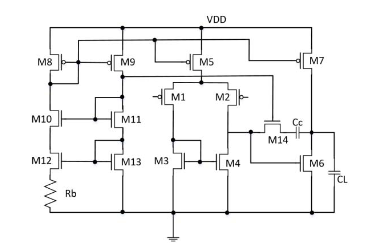
\includegraphics[width=6in]{images/TwoStageCMOSAMP.png} \\
\caption{The Two-Stage CMOS operational amplifier circuit\cite{opamp}}
\end{figure}

The operational amplifier that I found was from the \textit{Design and Analysis of Two-Stage CMOS Operational Amplifier for Fluorescence Signal Processing}\cite{opamp} paper. This was published in the IEEE in the Journal of Solid State Circuits. In this paper it describes a operational amplifier for use in fluorescent optical fiber temperature testing. The amplifier has a high common mode rejection ratio and low input offset voltage. 

\section{Problem 2}
\begin{quote}
Identify one operational amplifier that has been patented in
the past 5 years. Give the circuit schematic, patent number, and briefly
summarize the useful properties that the author claims for this circuit.

\end{quote}

The operational amplifier that I found was from Texas Instruments that is still pending from its application on 2023-02-16.



Schematic:\\
\begin{figure}[H]
\centering
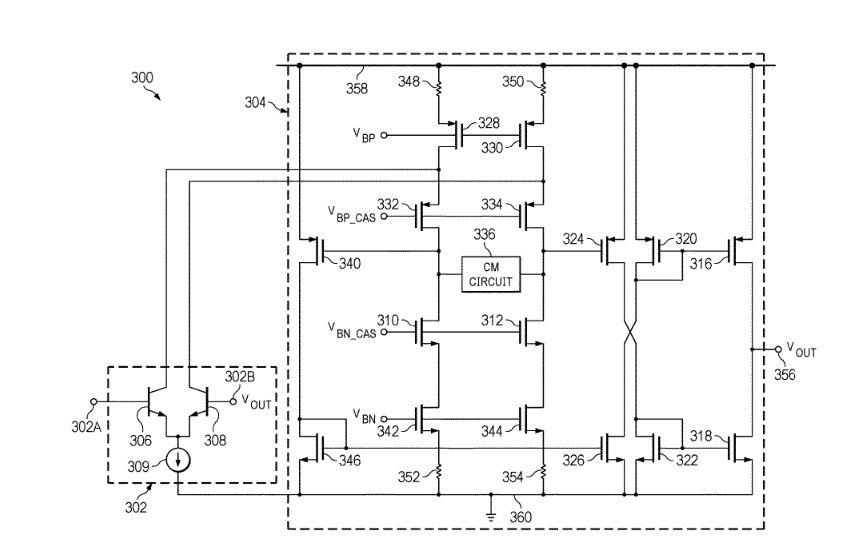
\includegraphics[width=6in]{images/TIOpAmpSchematic.png} \\
\caption{The operation amplifier schematic described in the TI patent\cite{patent}}
\end{figure}
Patent Number: US20230051462A1
Properties: The operational amplifier stresses the low quiescent current and a common mode voltage circuit (336). A more detailed schematic of the common mode (CM) circuit can be seen in figure 4 of the pattern or attached as figure \ref{CM}. It has a reversible current mirror to avoid stability issues (that come with low quiescent currents).

\begin{figure}[H]
\label{CM}
\centering

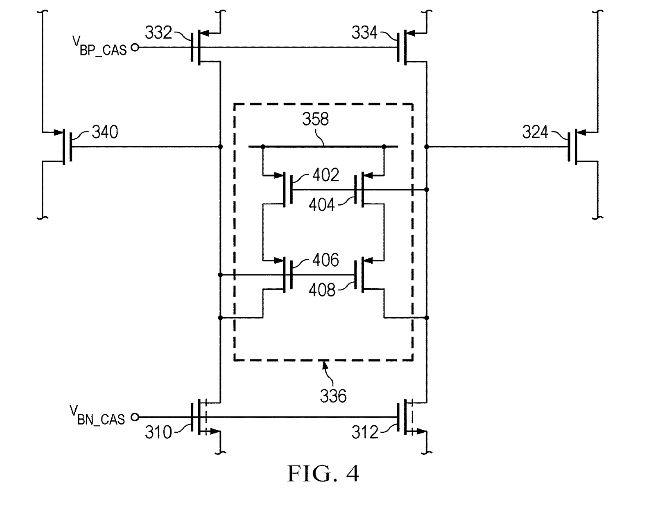
\includegraphics[width=3in]{images/TICMSchematic.png} \\
\caption{The common mode voltage control schematic described in the TI patent\cite{patent}}
\end{figure}



\section{Problem 3}
\begin{quote}
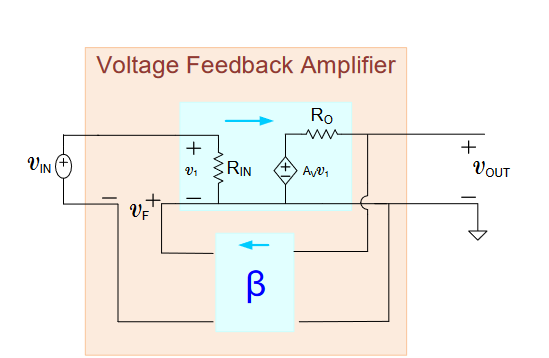
\includegraphics[width=6in]{images/problem3.png}\\

A block diagram of what is often termed a voltage-series feedback amplifier1 is shown below where it is assumed that the forward A amplifier is a voltage amplifier with an input impedance of RIN, an output impedance of R0 and a forward voltage gain of AV. The internal feedback amplifier, denoted with the symbol $\beta$, is assumed to be an ideal voltage amplifier (likely an attenuator) with infinite input impedance and zero output impedance with feedback signal \textbf{V} F = $\beta$ \textbf{V} OUT . The desensitivity, D, of a feedback amplifier is defined by the expression D = + A V $\beta$ . The voltage gain AV can itself be frequency dependent and modeled by the expression bandwidth of the forward amplifier.

Under these assumptions, show analytically that\\
\end{quote}

\subsection{Problem 3a}
\begin{quote}
a)The input impedance of the feedback amplifier is improved by D (i.e. RINF=RIN•D)\\
\end{quote}

\begin{multicols}{2}

In order for the effective input resistance to increase there are 2 things we can do. \\
1) Increase the Rin value (We cannot change this)\\
2) Decrease the current across Rin. (We can do this!)\\

When we add the feedback amplifier we are change the current draw from $\frac{V_{in} - 0}{R_{in}}$ to $\frac{V_{in} - V_f}{R_{in}}$. Because $V_f = \beta V_{out}$, we decreased the voltage drop and current flowing through $R_{in}$.\\


For the calculations I used this equation as a starting point.\\

\begin{equation}
\frac{V_{in}}{R_{inf}} = \frac{V_{in} - V_{f}}{R_{in}}
\end{equation}
Now rearranging we can get:\\
\begin{equation}
\frac{R_{inf}}{R_{in}} = \frac{V_{in}}{V_{in} - V_{f}}
\end{equation}

We can now solve for Vf in terms of Vin: 
\begin{equation}
\label{eq:VF}
V_f = \beta V_{out}
\end{equation}

\begin{equation}
\label{eq:VOUT}
V_{out} = A * V_1
\end{equation}

\begin{equation}
\label{eq:V1}
V_1 = V_{in} - V_f
\end{equation}

Substituting equation \ref{eq:V1} into equation \ref{eq:VOUT} we get\\

\begin{equation}
\label{eq:VOUT_VF}
V_{out} = A * (V_{in} - V_f)
\end{equation}
Lastly rearrange equation \ref{eq:VF} to\\

\begin{equation}
\label{eq:VOUT_VF2}
V_{out} =  \frac{V_f}{\beta}
\end{equation}

Combining the two VOUT equations we get
\begin{equation}
\label{eq:VF_VIN}
A * (V_{in} - V_f) =  \frac{V_f}{\beta}
\end{equation}

\begin{equation}
\label{eq:VF_VIN2}
A * V_{in} =  \frac{V_f}{\beta} + V_f *A
\end{equation}

\begin{equation}
\label{eq:VF_VIN3}
A * V_{in} =  V_f * (\frac{1}{\beta} + A)
\end{equation}

\begin{equation}
\label{eq:VF_VIN4VF}
V_f  =  V_{in} * (\frac{A * \beta}{1+ A * \beta})
\end{equation}

\begin{equation}
\label{eq:VF_VIN5}
\frac{R_{inf}}{R_{in}} = \frac{V_{in}}{V_{in} - V_{in} * (\frac{A * \beta}{1+ A * \beta})}
\end{equation}

\begin{equation}
\label{eq:VF_VIN6}
\frac{R_{inf}}{R_{in}} = \frac{1}{1 -  (\frac{D-1}{D})}
\end{equation}

\begin{equation}
\label{eq:VF_VIN7}
\frac{R_{inf}}{R_{in}} = \frac{D}{D - (D-1)}
\end{equation}

\begin{equation}
\label{eq:VF_RINF}
R_{inf} = D * R_{in}
\end{equation}
\end{multicols}


\subsection{Problem 3b}
\begin{quote}
b)The output impedance of the feedback amplifier is improved by D (i.e. ROF=RO/D)\\
\end{quote}
\begin{multicols}{2}

We can start with equations defining the output resistance. The output VOUT will be used to calculate Vf. We can set VIN to 0 while adding an output voltage (for KVL).

Add DC source to output as VOUT
\begin{equation}
V_{out} = I * R_{of} 
\end{equation}

KVL
\begin{equation}
AV_1 - V_{out} + I*R_o =0
\end{equation}

\begin{equation}
I = \frac{V_{out}- AV_1}{R_o}
\end{equation}

\begin{equation}
\frac{V_{out}}{R_{of}} = \frac{V_{out}- AV_1}{R_o}
\end{equation}

\begin{equation}
\frac{R_o}{R_{of}} = \frac{V_{out}- AV_1}{V_{out}}
\end{equation}

Short Vin
\begin{equation}
V_1 = -V_f
\end{equation}
\begin{equation}
V_out * B = V_f
\end{equation}

\begin{equation}
I = \frac{V_{out}+ BA V_{out}}{R_o}
\end{equation}

\begin{equation}
\frac{V{out}}{R_{of}} = \frac{V_{out}+ BA V_{out}}{R_o}
\end{equation}

\begin{equation}
\frac{1}{R_{of}} = \frac{1+ BA }{R_o}
\end{equation}

\begin{equation}
R_{of} = \frac{R_o}{D}
\end{equation}


\end{multicols}

\subsection{Problem 3c}
\begin{quote}
c)The closed loop bandwidth is improved by D (i.e. BWFB=BW*D)
\end{quote}
\begin{equation}
BW = \frac{A_v(s) * s}{A_{v0} - A_v(s)}
\end{equation}
A simple way of doing this is by recognizing the following formula
\begin{equation}
BW * Gain = unity gain bandwidth 
\end{equation}
Using equations 11 and 7 from part A we can calculate the VOUT/VIN
\begin{equation}
\frac{V_{out}}{V_{in}} = Gain = \frac{A}{D}
\end{equation}

Since these two values are inversely linked we can say that
\begin{equation}
BW_{FW} = BW *D 
\end{equation}

\subsection{Problem 3d}
\begin{quote}
d)The sensitivity of AFB with respect to AV has improved by D
\end{quote}
We proved this in equation 3 of part c. Gain goes down by a factor of D and so does sensitivity because they are interchangeable values.





\begin{quote}

Note: The improvements in this amplifier appear to be dramatic since the
desensitivity D can be very large. But the improvements might not be
quite as good as the calculations suggest since the assumptions of
ideality of the $\beta$ amplifier may be difficult to completely meet and
because it may be difficult to get perfect summing of VIN and VF. But in
good feedback designs, the improvements in these parameters can be
really significant.

Notation associated with feedback amplifiers is often a bit cumbersome
since the whole structure comprised of the ``A'' and ``$\beta$'' networks is
often called a feedback amplifier. And internal to this structure, there
is a ``$\beta$'' network which is an amplifier that provides a feedback signal
so it is often referred to as a feedback amplifier as well. In this
problem, the term ``feedback amplifier'' will refer to the whole
structure and ``local feedback amplifier'' will refer to the ``$\beta$''
network to avoid possible confusion.

\end{quote}

\section{Problem 4}
\begin{quote}
In the previous problem, feedback was used to build a voltage
feedback amplifier with improvements in four key characteristics.
Consider now the current feedback amplifier shown below where it is
assumed that the $\beta$ amplifier is an ideal current amplifier with zero
input impedance and infinite output impedance characterized by the
equation F = $\beta$ i OUT . The desensitivity is now defined by the
expression D = 1 + A I $\beta$ . Express RINF in terms of the desensitivity and the
parameters in the feedback amplifier and comment on these results relative to what was
obtained for the voltage feedback amplifier in the previous problem.
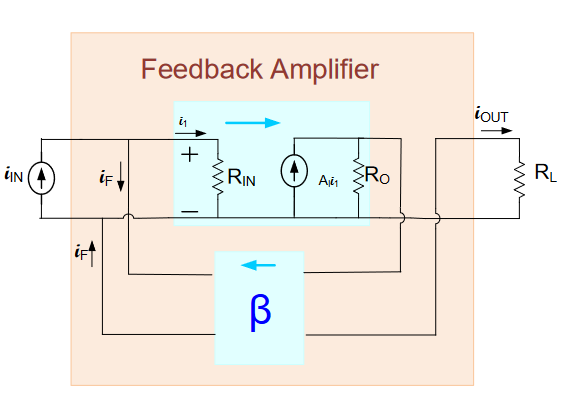
\includegraphics[width=2.99028in,height=1.71667in]{images/problem4.png}\\

\end{quote}

\begin{equation}
I_{in} R_{inf} = I_{1} R_{in}
\end{equation}
Now rearranging we can get:\\
\begin{equation}
\frac{R_{inf}}{R_{in}} = \frac{I_{1}}{I_{in}}
\end{equation}

We can now solve for I1 in terms of Iin and If: 
\begin{equation}
\label{eq:VF}
I_f = \beta I_{out}
\end{equation}

KCL
\begin{equation}
\label{eq:VOUT}
 A * i_1 - \frac{V_{o}}{R_o} - \frac{V_{o}}{R_L}
\end{equation}

\begin{equation}
\label{eq:VOUT}
V_{o} = \frac{A i_1 *(R_o R_L)}{R_o + R_L}
\end{equation}

\begin{equation}
\label{eq:VOUT}
I_{out} = \frac{V_{o}}{R_L}
\end{equation}


There should be no difference in Rin and Rinf. Based on the diagram the current that comes out of the beta block re-enters the beta block without interacting with the Rin.  

\section{Problem 5}
\begin{quote}
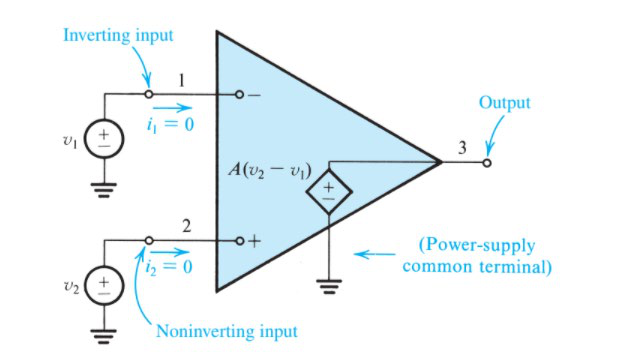
\includegraphics[width=2.99028in,height=1.71667in]{vertopal_3376d9a0695b4078a59040ba2f51c60d/media/image5.png}\\
In most texts, data sheets, and circuit schematics the
operational amplifier is represented as a 3-terminal device yet the
two-port model of an operational amplifier has 4 terminals (i.e. nodes)
as shown below. It thus appears that one terminal has somehow vanished
in the symbol or equivalently appeared in the two-port model.

Correspondingly, the model of the operational amplifier that is
described in the most recent version of the Sedra-Smith text shows four
terminals (one designated with the ground symbol) yet this ground
terminal does not appear to be on the op amp symbol or on the pinout of
the operational amplifiers we are using in the laboratory. Rigorously
reconcile this concept of the vanishing terminal!
\end{quote}

The 3 terminal device assumes that one of the vout connections is connected to ground. This can be seen in the ideal operational amplifier model where the vout is connected to gnd.\\

\begin{figure}[H]
\centering
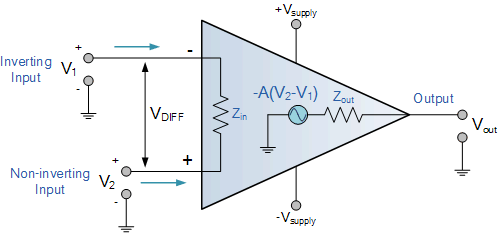
\includegraphics[width=2.99028in,height=1.71667in]{images/opamp1.png}
\caption{A model for an ideal operation amplifier\cite{opamp-pics}}
\end{figure}


Or even in schematics you can find this missing terminal. \\

\begin{figure}[H]
\centering
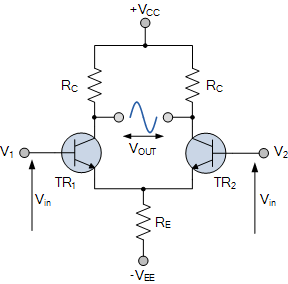
\includegraphics[width=2.99028in,height=1.71667in]{images/opamp-opamp52.png}\\
\caption{A schematic example for an operation amplifier\cite{opamp-pics}}
\end{figure}

This is normally set to ground but there are operational amplifiers with 4 terminal connections (differentiated output as well as input). Inversly there exists 2 terminal op amps as well! This was discussed in lecture. This can make sense as majority of use op amps has the positive terminal also connected to ground!


\section{Problem 6}
\begin{quote}
The actual op amp is a five-terminal device. After reconciling
this issue of the vanishing terminal in the previous problem, give an
expression for the nodal output voltage with respect to VSS for the
operational amplifier shown below which explicitly shows the 5 terminals
of the device.
\end{quote}
\begin{center}
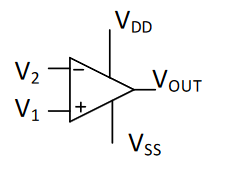
\includegraphics[width=4in]{images/problem6.png}\\
\end{center}
The first way I thought of this question was in a programming context. So if you had to model an operation amplifier, and while still keeping the ideal properties, I would use the following expression for the output.
\begin{lstlisting}
//OP AMP in C

Output_No_Power = Gain * (V1 -V2); //Output if supply voltage wasn't considered
VOUT = max(VSS, min(Output_No_Power, VDD));

\end{lstlisting}

Mathematically this could be represented as piece wise functions rather than code.


\section{Problem 7}
\begin{quote}

Two circuits that use a single operational amplifier are shown below.

a)Using the model of the standard model of the operational amplifier
that appears in the Sedra/Smith book, analyze the two circuits under the
assumption that the voltage gain of the op amp, AV, is finite.
\end{quote}
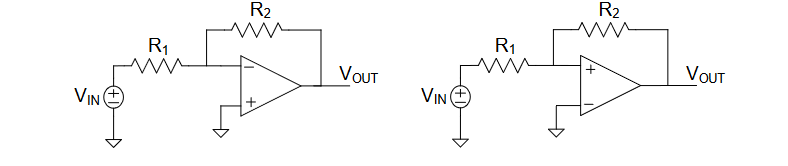
\includegraphics[width=6in]{images/problem7.png}\\

For the first circuit we can analyze with the following equations.

\begin{equation}
V_{out} = -A_v V_-
\end{equation}

\begin{equation}
V_- =  V_{in} + \frac{V_{out} - V_{in}}{R_1 + R_2} * R_1
\end{equation}

\begin{equation}
\frac{V_{out}}{-A_v} = V_{in} + \frac{V_{out} - V_{in}}{R_1 + R_2} * R_1
\end{equation}

\begin{equation}
V_{out} * (\frac{1}{A_v} + \frac{R_1}{R_1 +R_2}) = V_{in} * ( -1 + \frac{R_1}{R_1 + R_2})
\end{equation}

\begin{equation}
\frac{V_{out}}{V_{in}} =  \frac{-A_v *R_2}{A_v *R_1 + R_1 + R_2}
\end{equation}

For the second circuit we can analyze with the following equations.

\begin{equation}
V_{out} = A_v V_+ 
\end{equation}

\begin{equation}
V_+ = V_{in} + \frac{V_{out} - V_{in}}{R_1 + R_2} * R_1
\end{equation}

\begin{equation}
\frac{V_{out}}{A_v} = V_{in} + \frac{V_{out} - V_{in}}{R_1 + R_2} * R_1
\end{equation}

\begin{equation}
V_{out} * (\frac{1}{A_v} - \frac{R_1}{R_1 +R_2}) = V_{in} *( 1 - \frac{R_1}{R_1 + R_2})
\end{equation}

\begin{equation}
\frac{V_{out}}{V_{in}} =  \frac{-A_v *R_2}{A_v *R_1 - (R_1 + R_2)}
\end{equation}




b)Compare the voltage gain of the two circuits as the voltage gain AV
goes to $\infty$

Both configurations approach $\frac{-R_2}{R_1}$ as the gain approaches infinity.


\begin{quote}
c)Although an engineer should be able to analyze any interconnection of
basic devices and components, almost all basic electronics textbooks are
silent on the existence of the simple circuit on the right. Why is this
circuit is seldom discussed? Support your answer with sound analytical
principles or concepts.
\end{quote}

The secondary circuit is seldom discussed because it is not nearly as useful in analog circuits. This is because of the positive feedback in the design. We can see in the equation that the only difference between the two circuit gain equations is the bottom term $R_1+R_2$, it is either added or subtracted. When it is added it reduces the overall gain and slightly lowers the output voltage. If it is subtracted then it will be slightly greater. This is the problem. If it is slightly greater than the equation for $V_+$ shows that VOUT is linearly related. Any increase in this output voltage increases the input which in turn increases the output more. In the end the output voltage will clip at the rails at the slightest input. This small change ruins the stability of the circuit. What's actually very interesting is that we have proved that an ideal operational amplifier would not have a positive feedback issue because the infinite gain would remove this slight increase in gain.  


\section{Problem 8}
\begin{quote}
(Extra Credit)
One example was given in class where Conventional Wisdom does not correctly reflect reality and that was in describing the concept of the operational amplifier. Another example, also related to operational amplifiers, is the ``vanishing ground'' of Problem 5 in this homework assignment. See if you can identify another example, preferably in the electronics field, where Conventional Wisdom is not correctly aligned with reality.
\end{quote}

Another potential example where conventional wisdom fails is in server management. The conventional wisdom for building a server would be to have high end, extremely reliable parts in the goal of speed and maintaining user's data integrity. But when Google created their servers, they used cheap hardware prone to failure. Instead they use software and redundancy (possible because of savings on non high end parts) to maintain reliability while keeping costs lower with their large scale. In the Wikipedia's description of the Google File System (GFS) file system, it states that "It is also designed and optimized to run on Google's computing clusters, dense nodes which consist of cheap "commodity" computers, which means precautions must be taken against the high failure rate of individual nodes and the subsequent data loss."\cite{GFS} An interesting example of how you can get greater overall reliability with less reliable parts because of the difference in cost.





\begin{thebibliography}{9}
\bibitem{opamp}\href{https://ieeexplore.ieee.org/document/9532225}{Design and Analysis of Two-Stage CMOS Operational Amplifier for Fluorescence Signal Processing}
\bibitem{opamp-pics}\href{https://www.electronics-tutorials.ws/opamp/opamp_1.html
}{Operational Amplifier Basics}
\bibitem{patent}\href{https://github.com/Jetsama/EE435/blob/main/HW1/Sources/US20230051462A1.pdf}{TI Patent:Differential Amplifier Common Mode Voltage}
\bibitem{GFS}\href{https://en.wikipedia.org/wiki/Google_File_System}{Wikipedia: Google File System}

\end{thebibliography}

\end{document}
